
\documentclass[twocolumn]{aastex631}

\usepackage{amsmath}

\newcommand{\vdag}{(v)^\dagger}
\newcommand\aastex{AAS\TeX}
\newcommand\latex{La\TeX}
\newcommand{\red}[1]{\textcolor{red}{#1}}
\newcommand{\blue}[1]{\textcolor{blue}{#1}}
\newcommand{\CE}[1]{\textcolor{violet}{CE: #1}}

\begin{document}
	
\title{Physics inspired priors for neutron star mergers improves equation of state constraints}

\author[0009-0000-7037-1809]{Spencer J. Magnall}
\affiliation{School of Physics and Astronomy, Monash University, Clayton VIC 3800, Australia}
\affiliation{OzGrav: The ARC Centre of Excellence for Gravitational Wave Discovery, Clayton VIC 3800, Australia}


\author[0000-0002-8669-4300]{Christian Ecker}
\affiliation{Institut f\"ur Theoretische Physik, Max-von-Laue-Strasse 1, 60438 Frankfurt, Germany}

\author[0000-0002-1330-7103]{Luciano Rezzolla}
\affiliation{Institut f\"ur Theoretische Physik, Max-von-Laue-Strasse 1, 60438 Frankfurt, Germany}
\affiliation{Frankfurt Institute for Advanced Studies, Ruth-Moufang-Strasse 1, 60438 Frankfurt, Germany}
\affiliation{School of Mathematics, Trinity College, Dublin 2, Ireland}


\author[0000-0003-3763-1386]{Paul D. Lasky}
\affiliation{School of Physics and Astronomy, Monash University, Clayton VIC 3800, Australia}
\affiliation{OzGrav: The ARC Centre of Excellence for Gravitational Wave Discovery, Clayton VIC 3800, Australia}
	
\begin{abstract}
 Gravitational-wave astronomy shows great promise in determining nuclear physics in a regime not accessible to terrestrial experiments. 
 We introduce physics-inspired priors informed by nuclear theory and perturbative quantum chromodynamics calculations as well as astrophysical measurements of neutron star masses and radii.
 When these priors are used in gravitational-wave astrophysical inference, we show significant improvement on nuclear equation of state constraints. 
 Applying these to the first two gravitational-wave binary neutron star mergers GW170817 and GW190425, constraints on the radius of a $1.4\,M_\odot$ neutron star improves from $R=\red{XX^{+YY}_{-ZZ}}\,{\rm km}$ to $\red{XX^{+YY}_{-ZZ}}\,{\rm km}$ (90\% confidence intervals).
 We also show these priors can be used to perform model selection between binary neutron star and neutron star-black hole mergers, although the results for GW190425 are incolnclusive with a Bayes factor of $1.33$ in favour of the binary neutron star merger hypothesis, representing only marginal evidence.
 We advocate for these physics-inspired priors to be used as standard in the literature, and provide open-source code for reproducibility and further adaptation of the method.
 \CE{The abstract seems a bit optimisitc. Can we actually claim an improvement of the NS EOS and radius constraints?}
\end{abstract}
	
\keywords{neutron stars --- gravitational waves --- equation of state}
		
\section{Introduction} \label{sec:Intro}
	
\red{Some background sentences here on the  importance and constraints of pQCD and nuclear theory.}

When performing gravitational-wave astrophysical inference of binary neutron star mergers~\citep[e.g.,][]{abbott17_170817observation,abbott18_170817EOS,abbott19_170817Properties,abbott20_190425}, it is common to use `agnostic' priors on their gravitational-wave observables, for example, uniform priors on chirp mass $\mathcal{M}$ and the dimensionless tidal deformability parameter $\tilde{\Lambda}$. 
However, \citet{altiparmak22,Ecker:2022dlg} showed that the above conditions imply highly correlated probability distributions in $\mathcal{M}-\tilde{\Lambda}$ parameter space.
 	
In this work, we advocate using these physics-inspired priors joint priors on $\mathcal{M}$ and $\tilde{\Lambda}$, which are the two best measured and most informative parameters related to the neutron star equation of state (EOS).
We show an improvement on the measurement of the marginalized posterior on $\tilde{\Lambda}$ from the gravitational-wave observation of GW170817 from $\tilde{\Lambda}=\red{XX}$ with the agnostic prior to $\red{YY}$ with the new physics-inspired prior.
This corresponds to an improvement in the neutron star radius measurement of an equivalent $[1.4]\,{M_\odot}$ star from $\red{R_{1.4}}= $ to $\red{\ldots}$ \CE{How to quantify this improvement?}.
For GW190425, the improvement is \red{\ldots}.
	
We also demonstrate the utility of these priors for distinguishing between the sources of Gravitational wave events. 
We perform model selection between a binary neutron star and neutron star -- black hole origin of GW190425 and find a Bayes factor of \red{XX} in favor of a binary neutron star origin. 
	
In advocating for this prior becoming standard in the literature, we provide an open-source configuration for the \textsc{Bilby} Bayesian inference library~\citep{ashton19,romeroshaw20} currently used for the majority of gravitational-wave parameter estimation by the LIGO-Virgo-KAGRA collaboration~\citep{LIGO, Virgo, KAGRA}.
This implements numerically the joint probability distribution as a constrained prior for $\mathcal{M}$ and $\tilde{\Lambda}$ as described in the next section.
	
\section{Methods} \label{sec:Methods}
	
Our setup closely follows that of~\citet{Altiparmak:2022}, which we briefly review here. 
We begin by constructing a large set of EOSs by stitching together various components.
At the lowest densities ($n<0.5\,n_s$), with $n_s=0.16{\rm fm}^-3$ the nuclear saturation density, we adopt the Baym-Pethick-Sutherland (BPS) model~\citep{Baym71} for the neutron-star crust.
In the range $0.5\,n_s < n < 1.1\,n_s$, we randomly sample polytropes to span the range between the softest and stiffest EOSs from~\citet{Hebeler:2013nza}.
At high densities ($n \gtrsim 40\,n_s$), corresponding to a baryon chemical potential of $\mu = 2.6\,\rm GeV$, we impose the perturbative QCD constraint from~\citet{Fraga2014} on the pressure $p(X, \mu)$ of cold quark matter, with the renormalization scale parameter $X$ sampled uniformly in $[1,4]$.
	
For the intermediate density range ($1.1\,n_s < n \lesssim 40\,n_s$), we use the parametrization method of~\citet{Annala2019}, which models the sound speed as a function of the chemical potential, $c_s^2(\mu)$, using piecewise-linear segments:
\begin{equation} \label{eq:cs2}
 c_s^2(\mu) = \frac{\left(\mu_{i+1}-\mu \right) c_{s,i}^2 + \left(\mu - \mu_i \right) c_{s,i+1}^2}{\mu_{i+1}-\mu_i}\,, 
\end{equation}
where $\mu_i$ and $c_{s,i}^2$ are parameters defining the $i$-th segment in the range $\mu_i \leq \mu \leq \mu_{i+1}$.
Throughout this work, we adopt natural units where $c=G=1$.

The number density follows as 
\begin{equation} \label{eq:n}
 n(\mu) = n_1 \exp \left({\int_{\mu_1}^\mu \frac{d\mu^\prime}{\mu^\prime c_s^2(\mu^\prime)}}\right)\,, 
\end{equation} 
where $n_1 = 1.1\,n_s$, and $\mu_1 = \mu(n_1)$ is set by the corresponding polytropic EOS.
The pressure is then obtained via
\begin{equation} \label{eq:p}
 p(\mu) = p_1 + \int_{\mu_1}^\mu d\mu^\prime , n(\mu^\prime)~,
\end{equation}
where the integration constant $p_1$ matches the pressure of the polytrope at $n = n_1$.
We numerically integrate Eq.~\eqref{eq:p} using seven segments for $c_s^2(\mu)$.

Using this framework, we generate $\approx 10^6$ EOSs by randomly selecting the maximum sound speed $c_{s,{\rm max}}^2 \in [0,1]$ and uniformly sampling the free parameters $\mu_i \in [\mu_1, \mu_{N+1}]$ (where $\mu_{N+1} = 2.6\,\rm GeV$) and $c_{s,i}^2 \in [0, c_{s,{\rm max}}^2]$.
These EOSs are by construction consistent with nuclear theory and perturbative QCD uncertainties.

To incorporate astrophysical constraints, we solve the Tolman-Oppenheimer-Volkoff (TOV) equations for each EOS and retain only those satisfying the mass measurements of J0348+0432~\citep{Antoniadis2013} ($M = 2.01\pm 0.04\,M_{\odot}$) and J0740+6620~\citep{Cromartie2019, Fonseca2021} ($M = 2.08 \pm 0.07\,M_{\odot}$), discarding EOSs with a maximum mass $M_{\rm TOV} < 2.0\,M_{\odot}$. 
In addition, we impose NICER radius constraints from J0740+6620~\citep{Miller2021, Riley2021} and J0030+0451~\citep{Riley2019, MCMiller2019b}, rejecting EOSs with $R < 10.75\,\rm km$ at $M = 2.0\,M_{\odot}$ or $R < 10.8\,\rm km$ at $M = 1.1\,M_{\odot}$.
	
In the neutron star binary case, the binary tidal deformability is computed as
\begin{equation} 
 \tilde{\Lambda}_{\rm NSNS} = \frac{16}{13} \frac{ (12M_2 + M_1) M_1^4 \Lambda_1 + (12M_1 + M_2) M_2^4 \Lambda_2}{(M_1 + M_2)^5}\,,
\end{equation}
where $M_i$, $R_i$, and $\Lambda_i = \frac{2}{3} k_2 \left( R_i/M_i \right)^5$ ($i=1,2$) denote the component masses, radii, and tidal deformabilities, with $k_2$ being the second tidal Love number.
The chirp mass is given by $\mathcal{M}_{\rm chirp} = (M_1 M_2)^{3/5} (M_1+M_2)^{-1/5}$ and we in the following we will use the mass ratio defined as $q = M_2/M_1$.
	
In the mixed binary case, i.e., where one binary component is a neutron star and the other one a black hole, the formula for the binary tidal deformability simplifies, because black holes have zero tidal deformability $\Lambda_{\rm BH}=0$.
The binary tidal deformability in this case becomes
\begin{equation} 
 \tilde{\Lambda}_{\rm NSBH} = \frac{16}{13} \frac{ (12M_{\rm BH} + M_{\rm NS}) M_{\rm NS}^4 \Lambda_{\rm NS}}{(M_{\rm NS} + M_{\rm BH})^5}\,,
 \end{equation}
where $M_{\rm NS}$ and $\Lambda_{\rm NS}$ are the nuetron star mass and tidal defromability, respectively, and $M_{\rm BH}$ the black hole mass. 
The expressions for the chirp mass and mass ratio remain intact, with the understanding that $M_1=M_{\rm NS}$ and $M_2=M_{\rm BH}$. 
Unlike in~\citet{altiparmak22,Ecker:2022dlg} we do not impose any GW informed constraints on the binary tidal deformability in the construction of our proior.
	
	\subsection{Binary neutron star mergers}
	We use the probability distribution of $10^7$ equation of state models informed by nuclear physics, perturbative quantum chromodynamics and  astrophysics from~\citet{altiparmak22} to generate a probability distribution for chirp mass -- tidal deformability, and use it as priors on those quantities as shown in Fig.~\ref{fig:priors}. We implement this in \textsc{Bilby} using the \verb!conditional_prior! function\footnote{\red{git link to our code!?}},
	interpolating the $200\times200$ grid to draw from a joint prior on $\mathcal{M}$ and $\tilde{\Lambda}$. 
	\begin{figure}
		\centering
		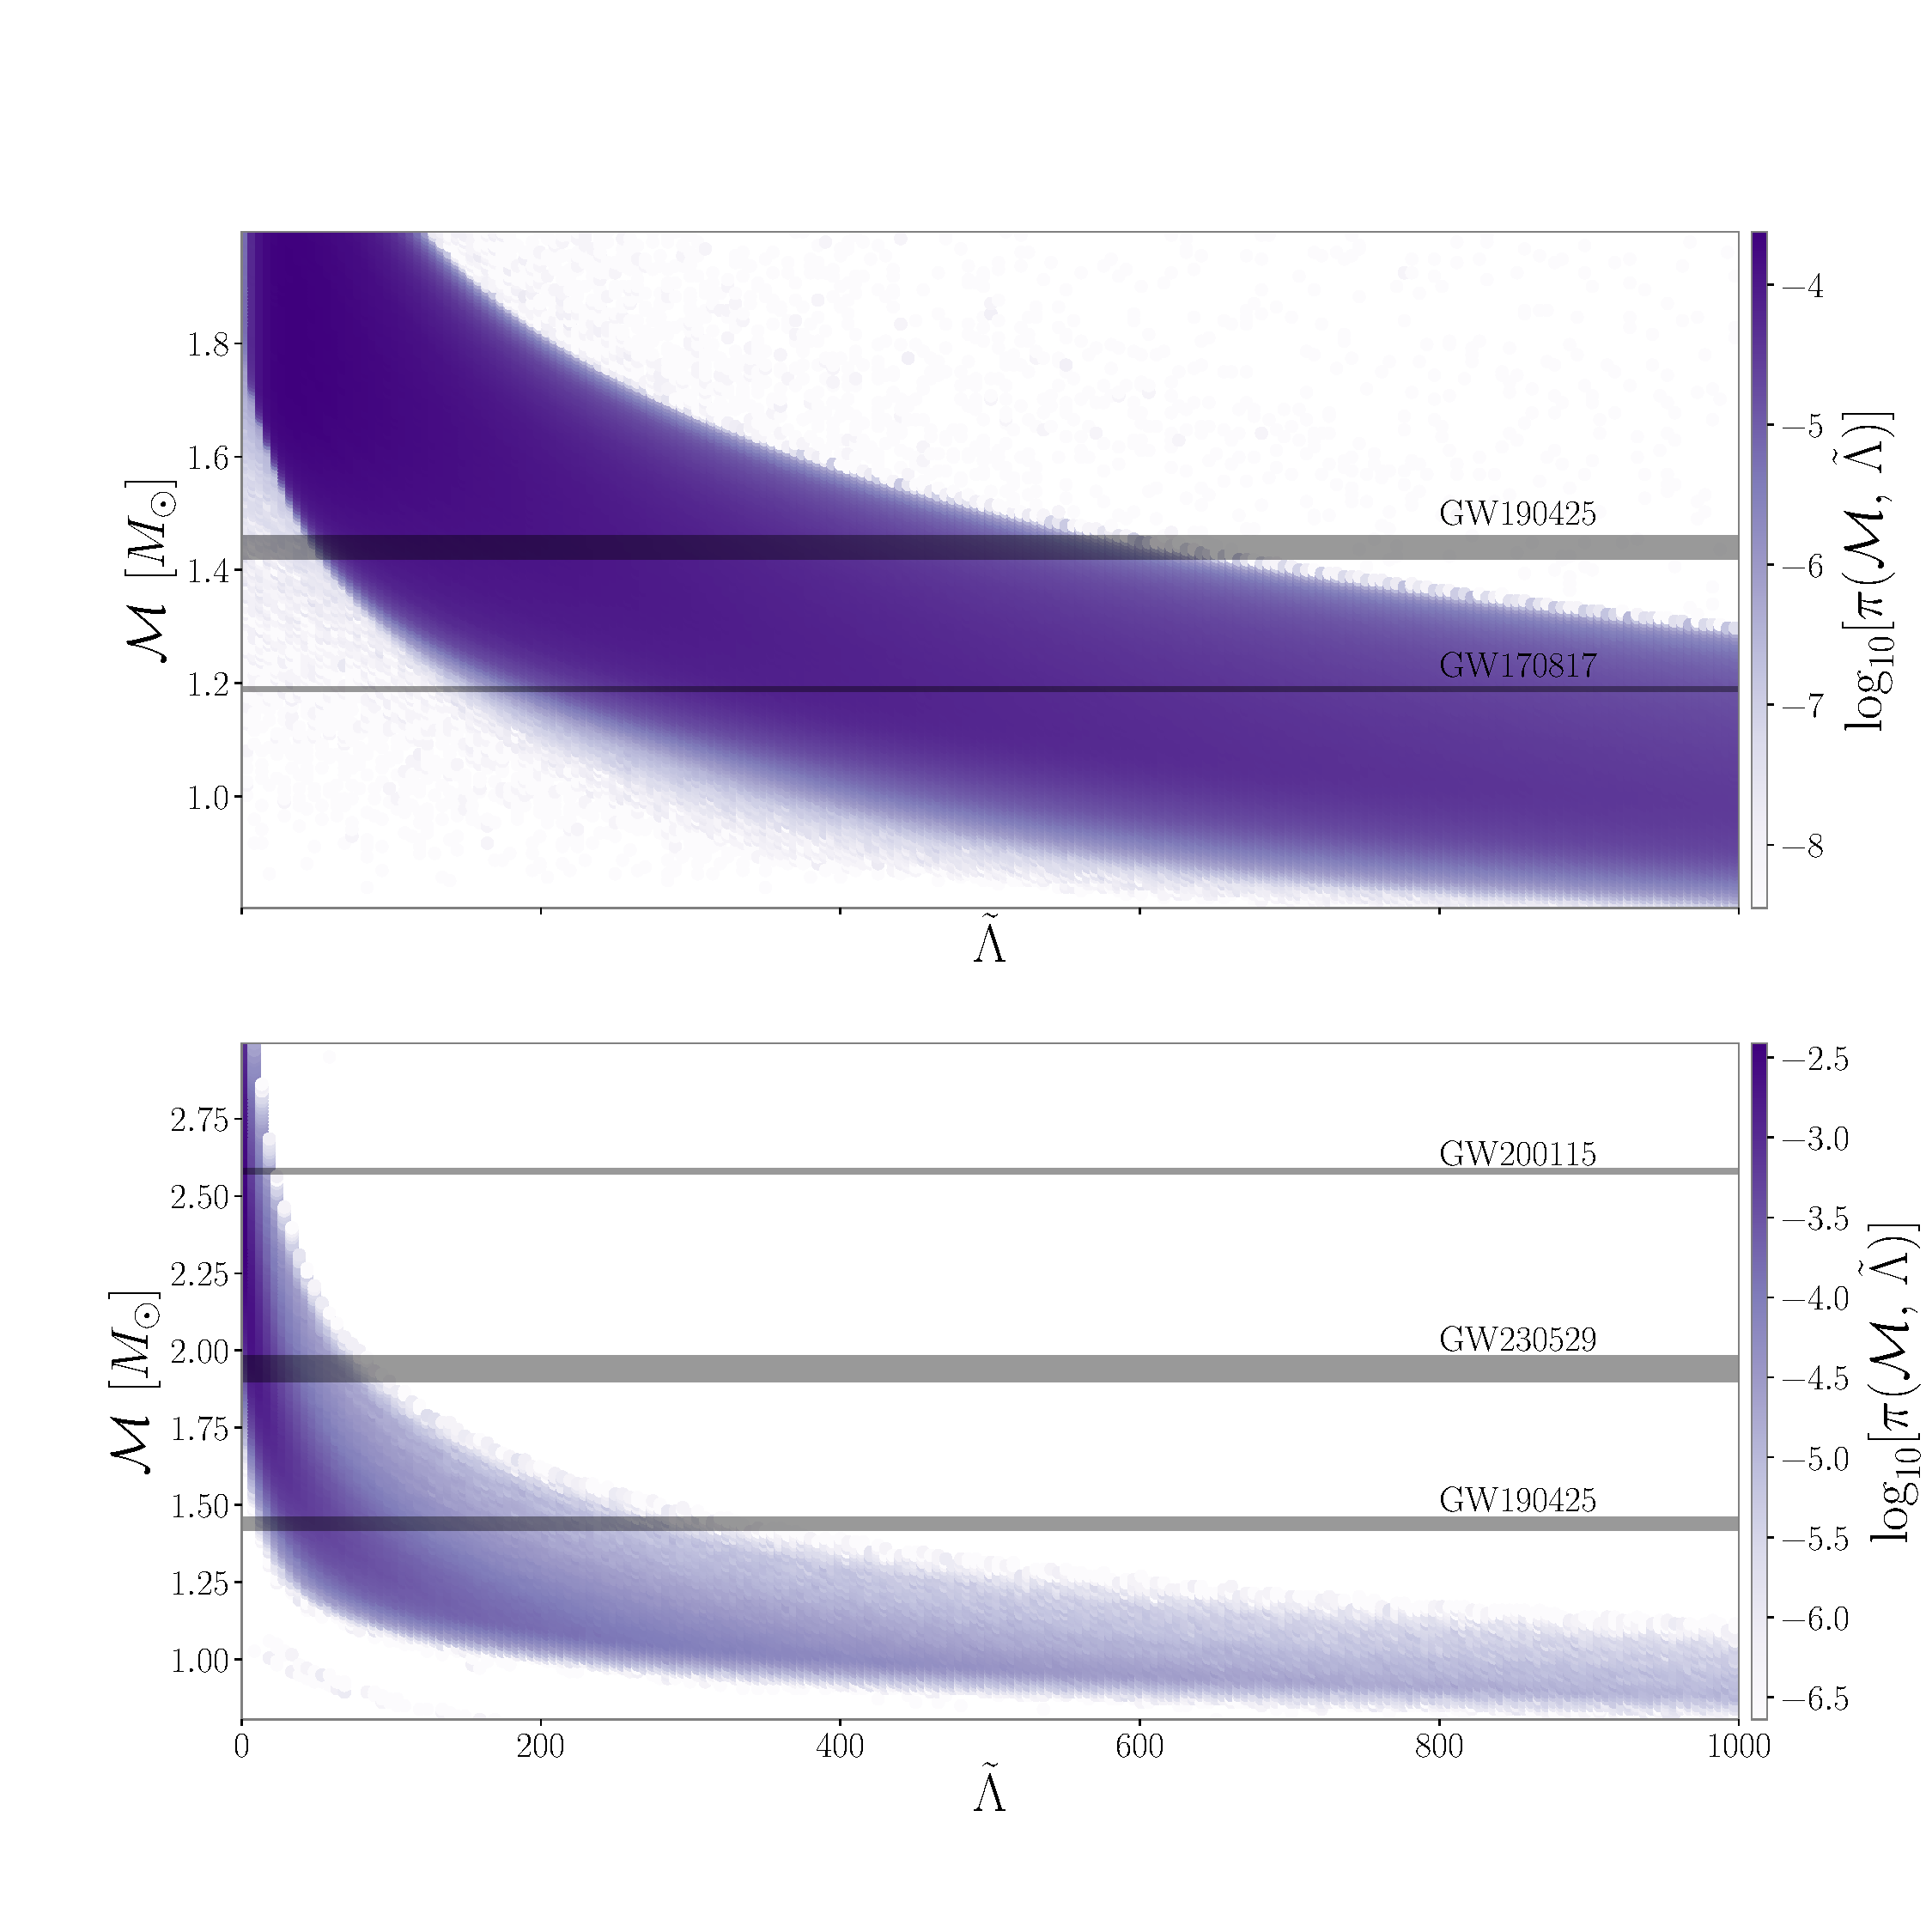
\includegraphics[width=1.\linewidth]{Fig_1_Physics_priors.pdf}
		\caption{Coupled priors for the source-frame chirp mass $\mathcal{M}$ and dimensionless tidal deformability $\tilde{\Lambda}$. Top: prior for binary neutron star mergers. Bottom: prior for neutron star -- black hole mergers. The horizontal grey bands are the 90\% credible intervals for the measured chirp masses of GW170817~\citep{abbott17_170817observation}, GW190425~\citep{abbott20_190425}, GW200115~\citep{GW200115} and GW230529~\citep{GW230529}}. 
		\label{fig:priors}
	\end{figure}
	
	We sample directly in source-frame chirp mass, mass ratio $q=m_1/m_2$ and the two tidal deformability parameters $\tilde{\Lambda}$ and $\delta\Lambda$~\citep[see][for explicit expressions for these quantities]{favata14,wade14}. We note that $q$ is not a variable that depends on the equation of state, but instead priors \textit{could} be chosen based on astrophysical formation scenarios. In this work, we take the standard approach and choose a prior on $q$ that is uniform between $q=0.125$ and 1~\citep[e.g.,][]{romeroshaw20}.
	
	We further note that, while both $\tilde{\Lambda}$ and $\delta\tilde{\Lambda}$ are related to the equation of state, we only impose a prior here on $\tilde{\Lambda}$. In general, $\tilde{\Lambda}$ is measured much better than $\delta\tilde{\Lambda}$, which can be understood because $\tilde{\Lambda}$ enters waveform approximates at the $5^{\rm th}$ post-Newtonian order, whereas $\delta\tilde{\Lambda}$ only enters at $6^{\rm th}$ in linear combination with $\tilde{\Lambda}$~\citep{wade14}. In principle, one could set a combined prior on the three parameters $(\mathcal{M},\,\tilde{\Lambda},\,\delta\tilde{\Lambda})$, however, adding this latter parameter would not add significantly to parameter estimation in the relatively low signal-to-noise regime because of the above arguments.
	
	
	\subsection{Neutron star -- black hole mergers}
	The parameterisation in the previous section does not go to high enough values of chirp mass because it is assumed both stars in the merger are neutron star. We therefore derive a new distribution for neutron star--black hole mergers by going back to the raw distributions of progenitor stellar masses and radii, and combining that progenitor with a black hole of mass $m_1$ and tidal deformability $\Lambda_1=0$.
	We use a uniform  distributed mass ratio to generate our prior relationship. We have found more sophisticated mass-ratio distributions, such as those informed by state of the art binary population synthesis (e.g \citealt{2021Broekgaarden+}) did not significantly impact the shape of the prior distribution. We demonstrate the independence of our results on the chosen population model in Appendix~\ref{sec:NSBH generation}. 
	We choose once again to work with priors in $\mathcal{M}$ -- $\tilde{\Lambda}$, enforcing $\tilde{\Lambda}(\Lambda_2,\mathcal{M},q)$ where $\Lambda_2$ is the tidal deformability of the lighter object in the binary, which we assume is the neutron star.
	\subsection{Parameter estimation}
	We perform Bayesian parameter estimation on the Gravitational-Wave strain data of the two (likely) binary neutron star merger events GW170817 and GW190425 using the strain data freely available from the GWOSC repository~\footnote{\url{https://gwosc.org}}. 
	We utilize the \textsc{Bilby} Bayesian inference framework and priors on source--frame chirp mass and tidal--deformability implemented in Section \ref{sec:Methods}. Priors for all renaming parameters assume the low-spin ($\chi \leq 0.05$) defaults as defined in \textsc{Bilby} (e.g \citealt{ashton19}, \citealt{romeroshaw20}).
	
	Parameter estimation for each run was performed using the \textsc{dynesty} nested sampler~\citep{Dynesty} and the \textsc{IMRPhenomPv2\_NRTidal} waveform~\citep{IMRPhenomP_NRtidal}. Analysis of binary neutron star merger signals is significantly computationally expensive and as such we utilize \textsc{pBilby}~\citep{pbilby}, a parallel implementation of \textsc{Bilby} which uses the Message Passing Interface (MPI). 
	
	Since we are required to sample in the source--frame chirp mass instead of the observer frame, we must assume a cosmology. We use $H_0=67.66 \rm  \ km  \ s^{-1}$, $\Omega_M = 0.30966 $ informed by the Planck 2018 results~\citep{Planck}.  
	
	We employ both the binary neutron star and the neutron star -- black hole merger priors in our analysis of GW190425. This facilitates a model selection analysis between a binary neutron star, and neutron star -- black hole origin of GW190425. The details of this model selection analysis are described further in Appendix \ref{sec:Model Selection}. 
	For GW170817 we perform parameter estimation using the binary neutron star prior only. 
	
	We reconstruct mass--radius curves from posterior samples of source--frame chirp and tidal deformability using \red{\ldots}
	
	
	\section{Results} \label{sec:Results}
	
	
	\subsection{GW170817}
	Figure \ref{fig:GW170817_tides} shows the posterior distributions of intrinsic tidal parameter of GW170817 analyzed using the $\mathcal{M}-\tilde{\Lambda}$ feature (teal), when compared to the official posterior samples from the LVK (midnight blue). While we show only the tidal posteriors, we sample over all binary parameters. \red{The full posteriors for this event are shown in Appendix XX}. 
	
	Figure \red{XX} shows the reconstructed mass---radius curves of GW170817 ... 
	\subsection{GW190425}
	Figure \ref{fig:GW190425_tides} shows the posterior distribution of the intrinsic tidal parameter of GW190425 when analyzed using both the binary neutron star prior (teal) and neutron star -- black hole prior (pink). We show the official posterior distribution  of the LVK obtained using uniform priors in blue. 
	% Z_BNS = -576535.277281933
	% Z_NSBH = -576535.5652987232
	Bayesian model selection between the binary neutron star and neutron star -- black hole merger gives a Bayes factor of 1.33, marginally in favor of a binary neutron star merger origin. 
	Figure \red{XX} shows the reconstructed mass radius curves of GW190425 analyzed using the new priors.  
	\begin{figure}
		\centering
		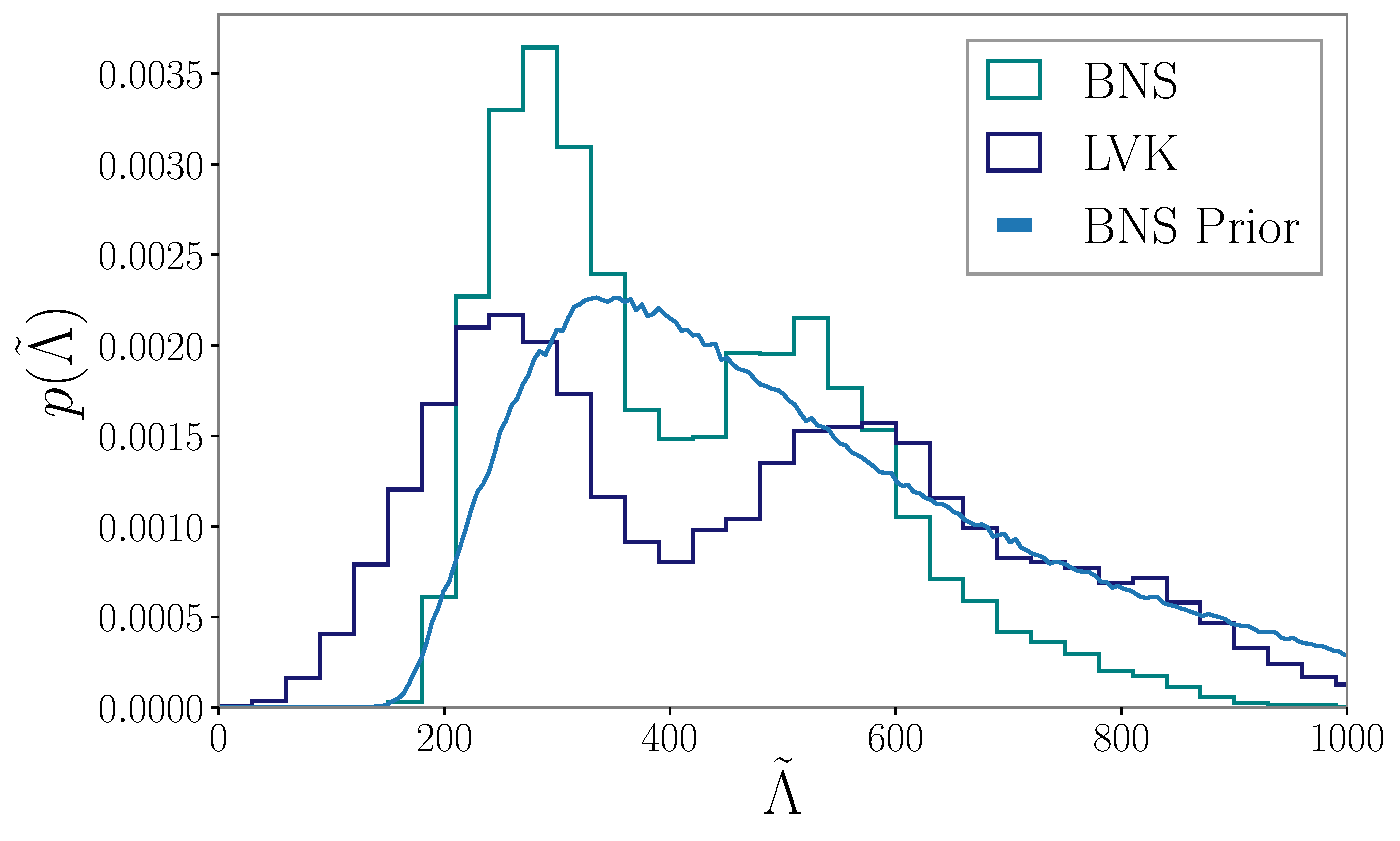
\includegraphics[width=1.\linewidth]{Fig_2_GW170817_lambda_tilde_posteriors_BNS.pdf}
		\caption{The posterior distributions of the tidal deformability $\tilde{\Lambda}$ obtained from Bayesian parameter estimation for GW170817. The posterior using a nuclear, microphysics, and astrophysics inspired prior is shown in teal, while the posterior using uniform priors from the LVK is shown in midnight blue. We show the (marginalized) prior with the light blue curve. Note, the posterior samples from the LVK show support up to $\tilde{\Lambda}$ = 2000. }
		\label{fig:GW170817_tides}
	\end{figure}
	
	\begin{figure}
		\centering
		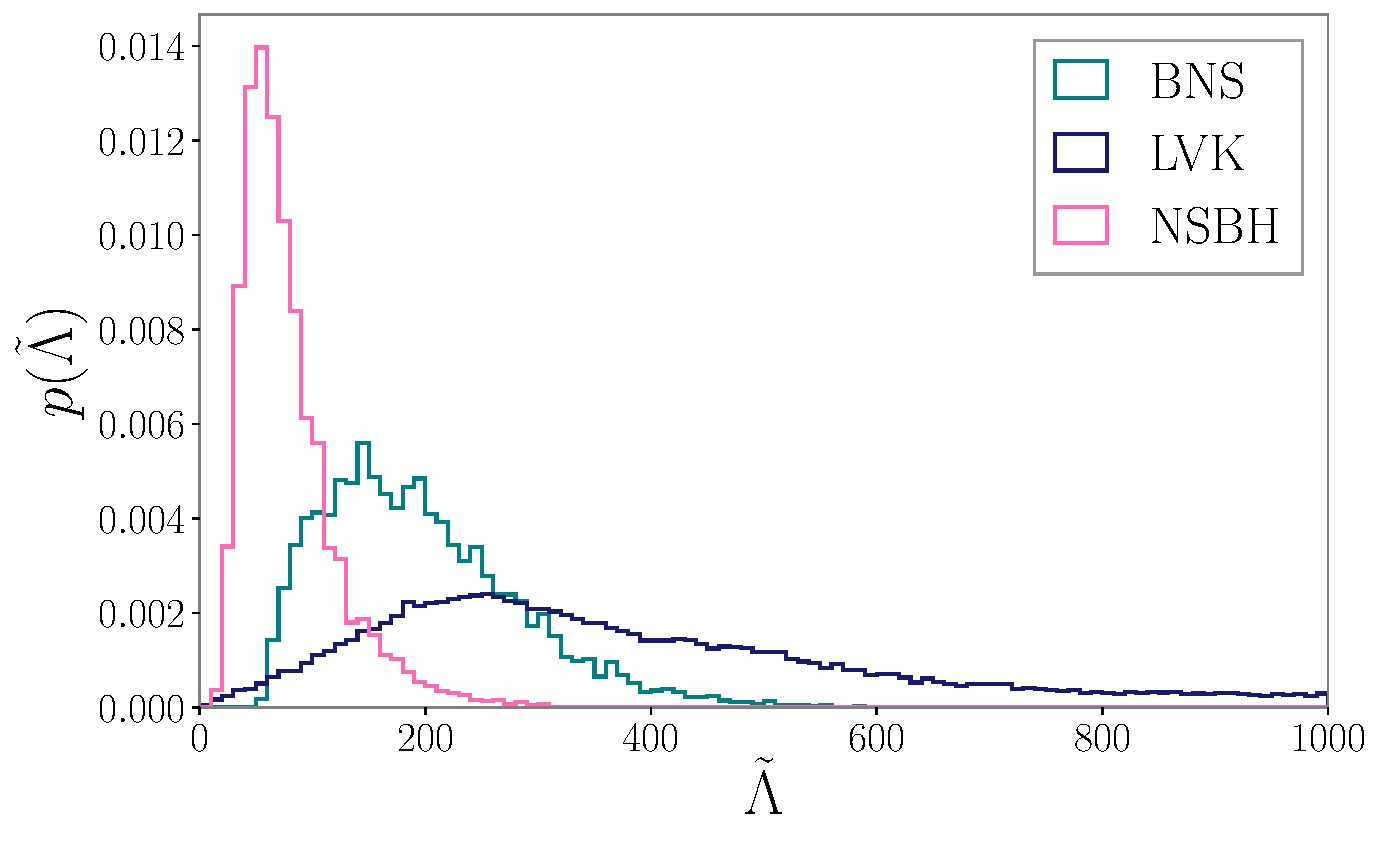
\includegraphics[width=1.\linewidth]{Fig_3_GW190425_lambda_tilde_posteriors.pdf}
		\caption{The posterior distributions of the tidal deformability $\tilde{\Lambda}$ obtained from Bayesian parameter estimation for G190425. The posterior using a nuclear, microphysics, and astrophysics inspired binary neutron star prior is shown in teal, and the corresponding neutron star --~black hole prior is shown in pink. 
			The posterior using uniform priors from the LVK is shown in midnight blue. }
		\label{fig:GW190425_tides}
	\end{figure}
	
	\section{Conclusions}
	
	\appendix
	
	\section{Neutron star -- black hole merger prior generation}\label{sec:NSBH generation}
	
	\red{We should detail the prior generation for neutron star -- black hole here, in particular the independence of a mass ratio informed by population synthesis on the prior distributions and potentially the resultant posterior distributions. Might be worth showing an extreme example to prove the point.}
	
	We generate two relations, one with uniform priors on our population of BH - NS mergers, and one directly informed by state of the art binary population synthesis. We use the mass ratio distribution of \cite{2021Broekgaarden+}  (\red{ what particular model are we using?}) for the generation of our population synthesis informed priors. Figure \ref{fig:mass ratio distrbution} shows the distribution in mass ratio used for the generation of the prior. 
	\begin{figure}
		\centering
		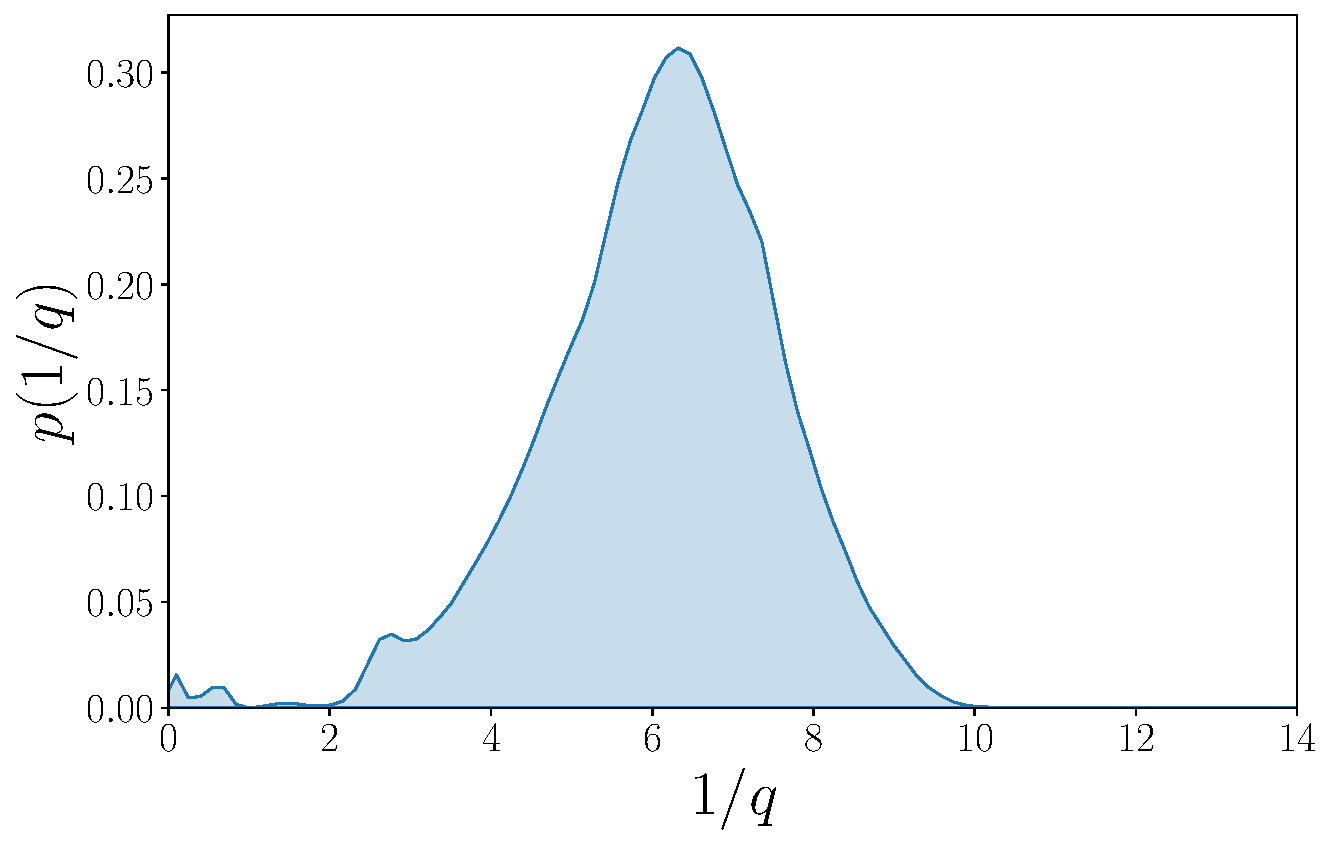
\includegraphics[width=\linewidth]{NSBH_mass_ratio_density.pdf}
		\caption{Probability density function of the mass ratio for detectable neutron star black hole mergers from \citep{2021Broekgaarden+}.}
		\label{fig:mass ratio distrbution}
	\end{figure}
	\section{Model Selection}\label{sec:Model Selection}
	We perform parameter estimation of gravtitational-wave strain data using the \textsc{dynesty} nested sampler. Unlike standard MCMC samplers,
	\textsc{dynesty} calculates the evidence for each parameter estimation run.   
	To perform Bayesian model selection between binary neutron star and neutron star-- black hole mergers, we calculate the Bayes factor
	\begin{equation}
		\rm BF  = \frac{\mathcal{Z_{\rm BNS}}}{\mathcal{Z_{\rm NSBH}}},
	\end{equation}
	where $\mathcal{Z}_{\rm BNS}$ and $\mathcal{Z}_{\rm NSBH}$ are the Bayesian evidences obtained for the parameter estimation runs using the binary neutron star 
	and neutron star black hole priors respectively.
	%  In practice we compute the log Bayes factor
	% \begin{equation}
	% 	\log \ (\rm BF) = \log (Z_{\rm BNS} ) - \log (Z_{\rm NSBH}).
	% \end{equation} 
	Formally, for model selection we should be computing the odds ratio, which is defined as
	\begin{equation}
		\mathcal{O} \equiv \frac{Z_{\rm BNS}}{Z_{\rm NSBH}} \frac{\pi_{\rm BNS}}{\pi_{\rm NSBH}},
	\end{equation}
	where $\pi_{\rm BNS}$ and $\pi_{\rm NSBH}$ are the prior odds for each hypothesis; i.e our relative belief about which hypothesis is more likely. 
	In this work we set the prior odds to unity, so the odds ratio is the Bayes factor. 
	We could in principle construct an odds ratio where the prior odds was informed by the relative rates of binary neutron star and neutron -- star black hole mergers. 
	However since these rates are still highly uncertain, we choose the more agnostic approach of setting the prior odds to unity. 
	\bibliography{references}{}
	\bibliographystyle{aasjournal}
	
	
\end{document}

